%!TEX program = xelatex
%!TEX TS-program = xelatex
%!TEX encoding = UTF-8 Unicode
\documentclass[aspectratio=169]{beamer}
\usepackage[UTF8, heading = false, scheme = plain]{ctex}
\usepackage{silence}
\WarningFilter{biblatex}{Patching footnotes failed}
\usepackage[hyperref=true,backend=biber,sorting=none,backref=true,style=ieee]{biblatex}
\addbibresource{references.bib}
\renewcommand{\footnotesize}{\tiny}
\usepackage{graphicx}
\usepackage{subfig}
\usepackage{caption}
\captionsetup{font={scriptsize}}
% \usepackage{tikz}

% \usetheme{Madrid}

% \titlegraphic{
\includegraphics[width=2cm, height=2cm]{fig/jnulogo.png}}
\title{去中心化深度学习的隐私保护研究}
% \author{
\includegraphics[width=2cm, height=2cm]{fig/jnulogo.png}}
\author{熊凯亚}
\date{\today}
\institute[JNU]{Jinan University}


\begin{document}

\begin{frame}
\titlepage
\end{frame}

% \addtobeamertemplate{frametitle}{}{%
% \begin{tikzpicture}[remember picture,overlay]
% \node[anchor=north east,yshift=2pt] at (current page.north east) {
\includegraphics[height=1cm]{fig/jnulogo.png}};
% \end{tikzpicture}}

\begin{frame}{Outline}
\tableofcontents
\end{frame}

\section{引言}
\begin{frame}{引言}

最近看了一些关于在去中心化的深度学习场景下的隐私保护的文章。去中心化的深度学习主要有两个方向:\tabularnewline
\begin{itemize}
\item CCS'15上Shokri等人\cite{shokri2015privacy}提出的隐私保护多方参与的协作深度学习模型(Collaborative Deep Learning)\footfullcite{shokri2015privacy}
\item Google 提出的针对移动设备(Android)的多方参与的\href{https://research.googleblog.com/2017/04/federated-learning-collaborative.html}{联合学习}(Federated Learning)\footnote{联合学习:https://research.googleblog.com/2017/04/federated-learning-collaborative.html}

\end{itemize}
\end{frame}

\begin{frame}{引言}{协作深度学习}
\begin{figure}
\begin{tabular}{cc}
\subfloat[传统的中心化学习]{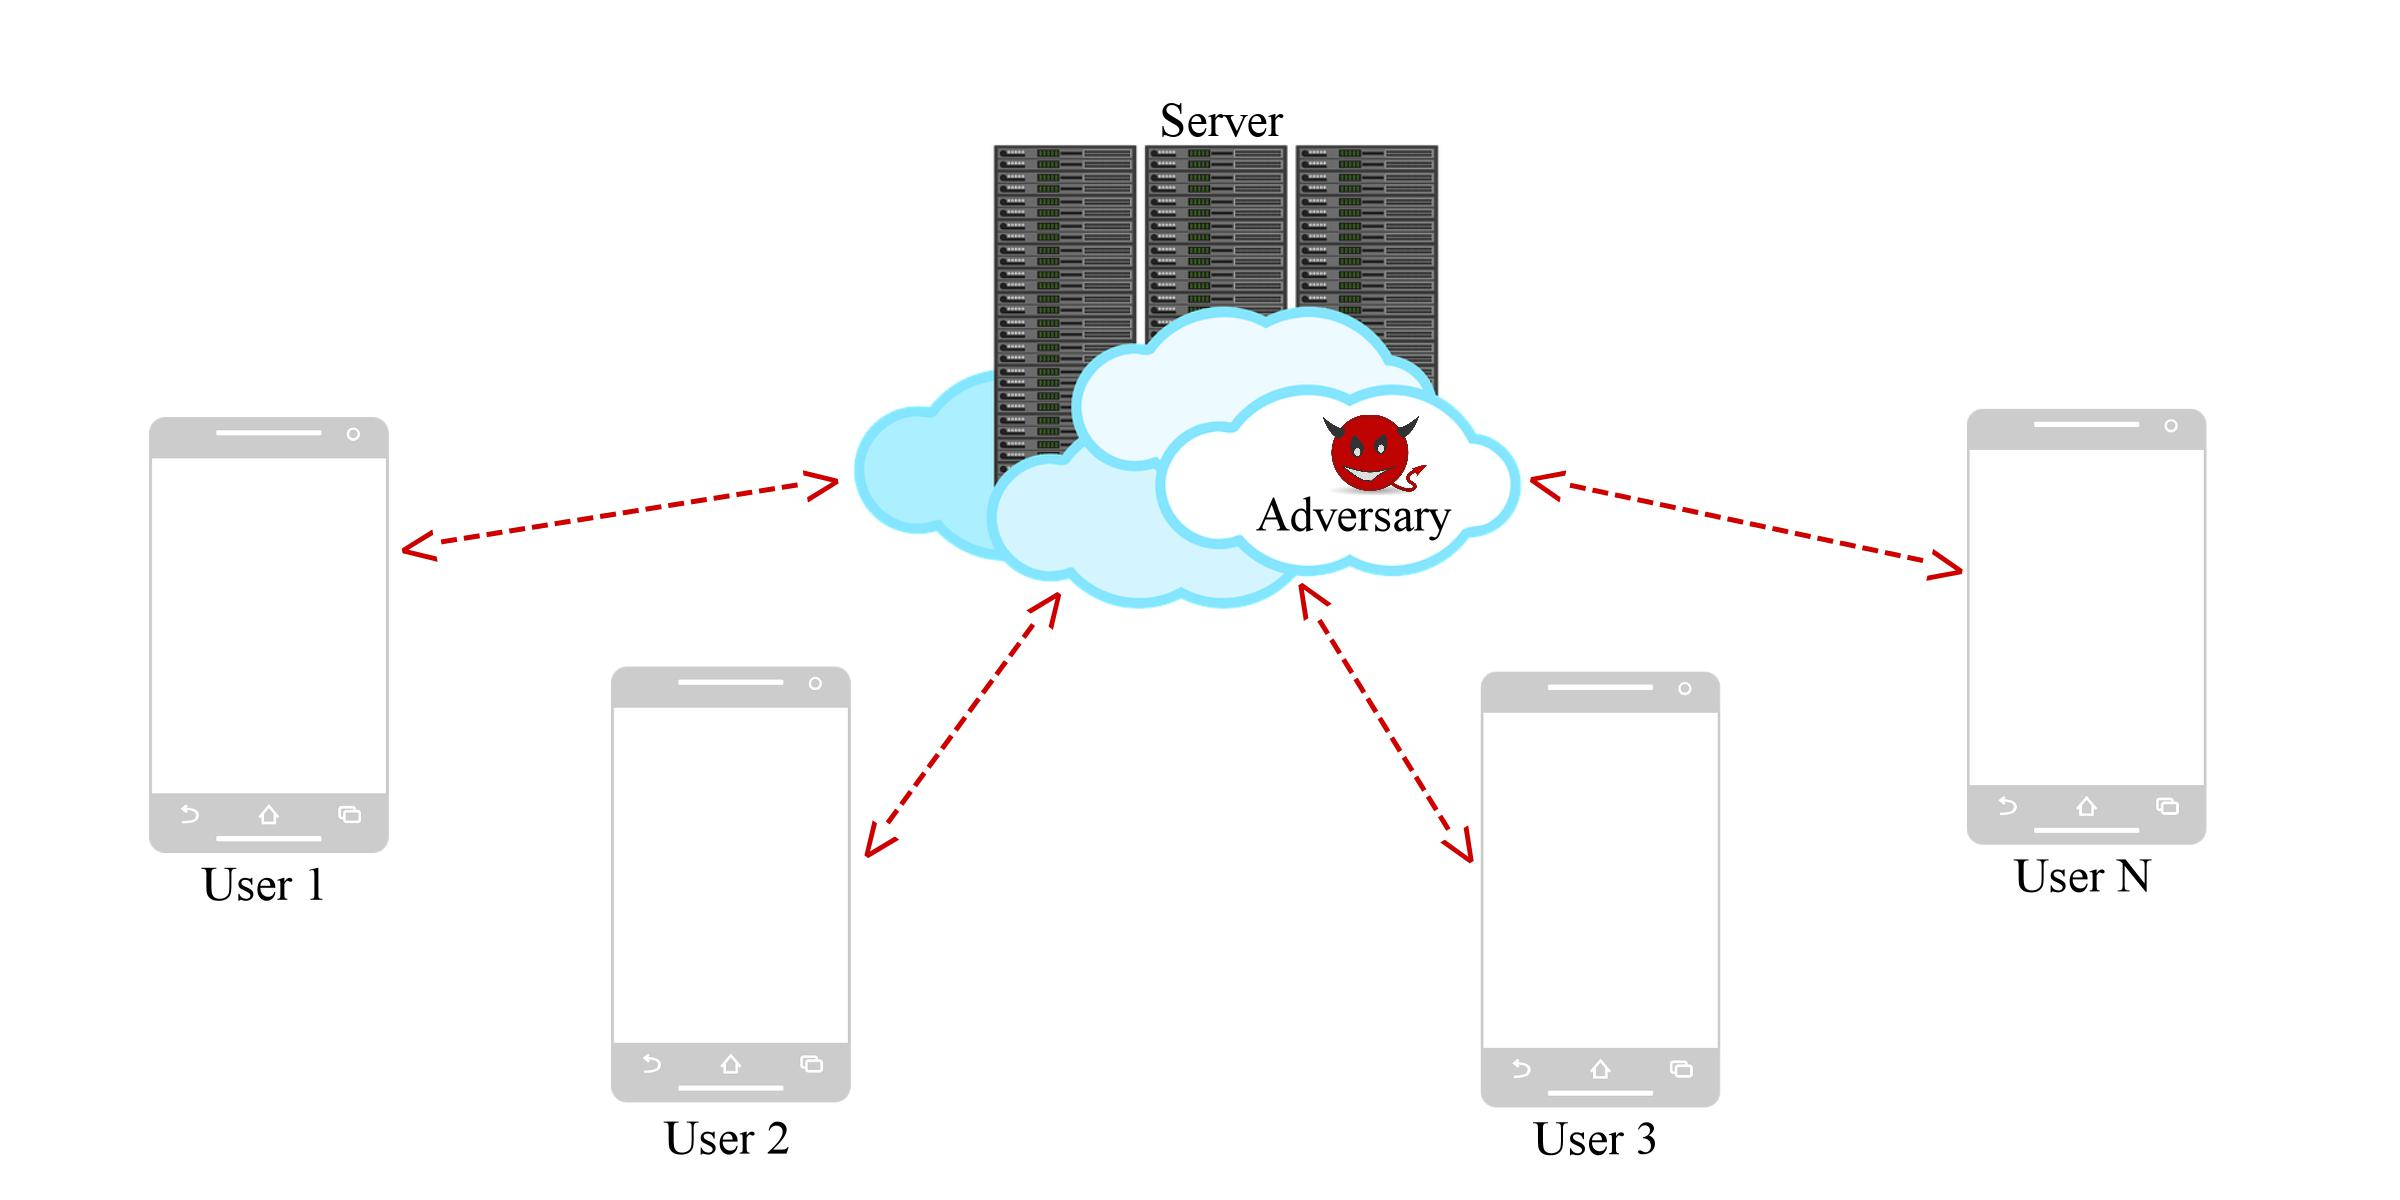
\includegraphics[width = 2.5in]{fig/scenario_1}} &
\subfloat[去中心化学习]{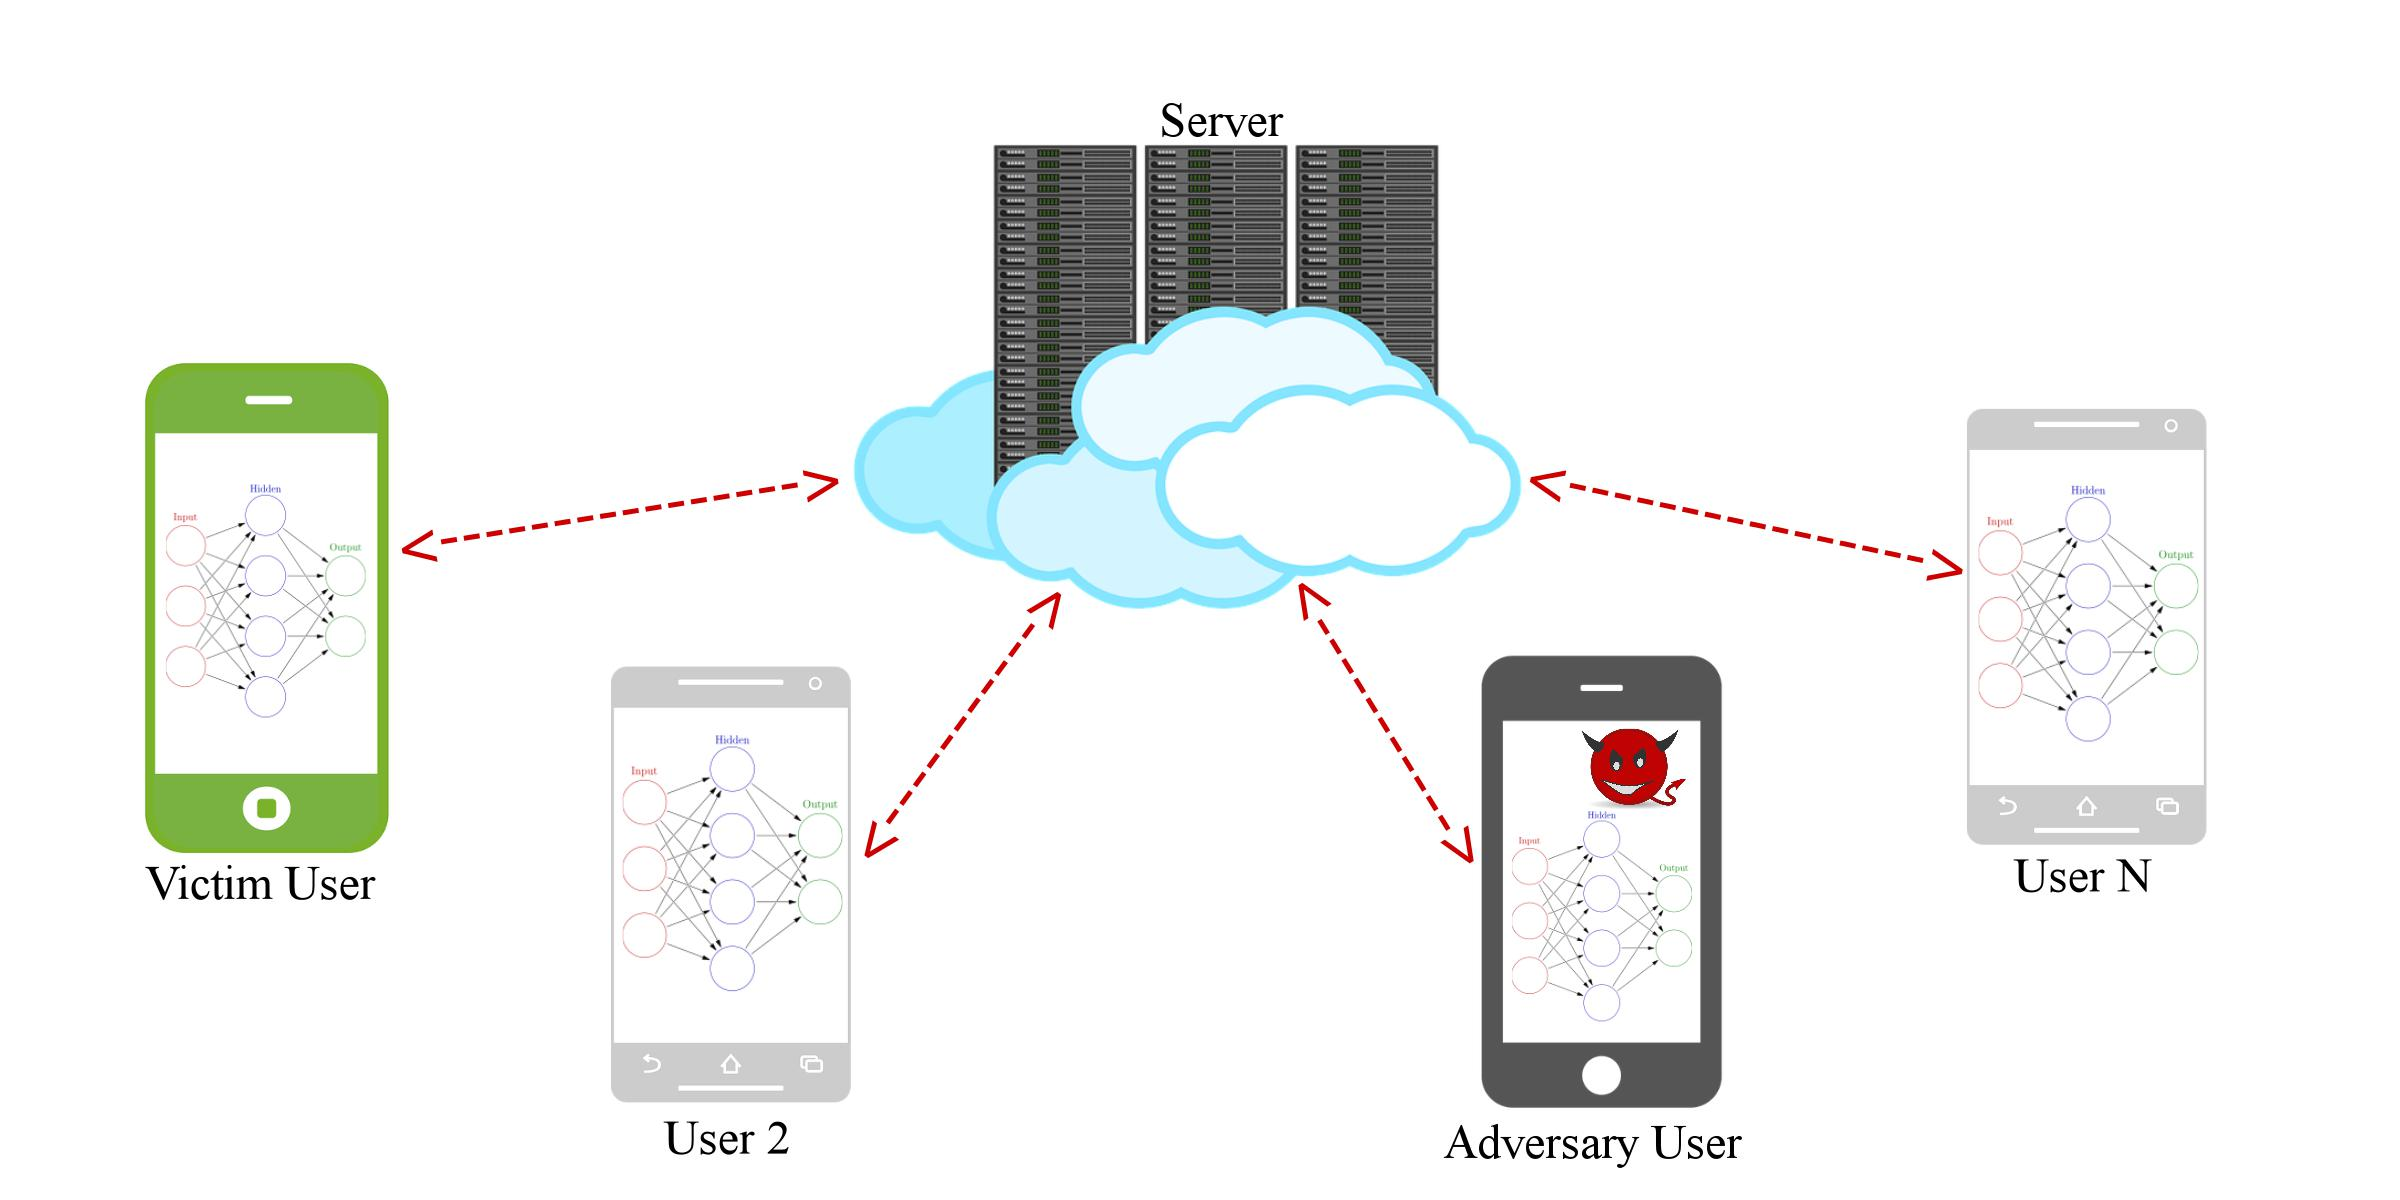
\includegraphics[width = 2.5in]{fig/scenario_2}}
\end{tabular}
\caption{传统中心化学习和去中心化学习对比}
\label{fig:learningApproaches}
\end{figure}
\end{frame}

\begin{frame}{引言}{联合学习}
\begin{figure}[!ht]
\centering
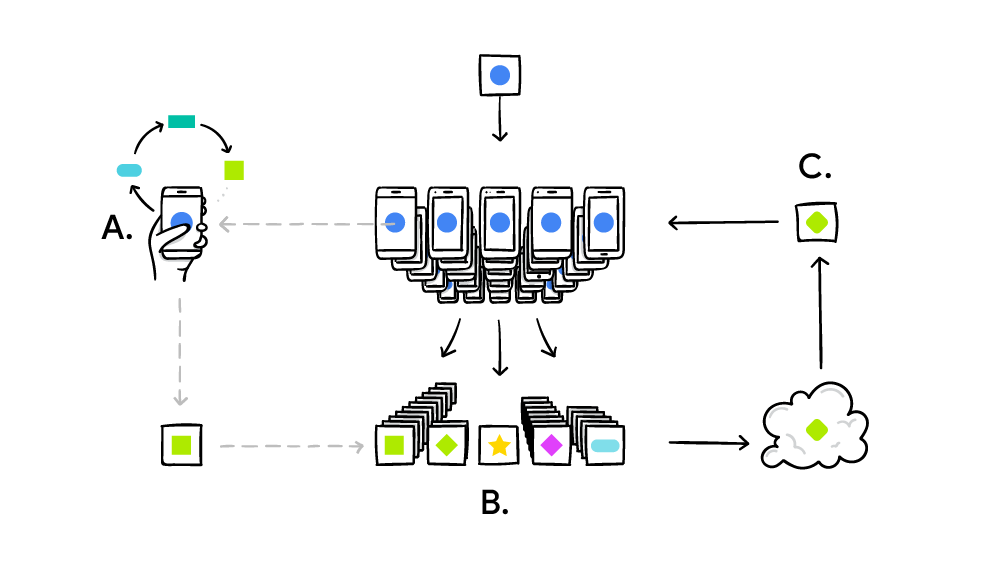
\includegraphics[width = 4in]{fig/FederatedLearningFlow}
\caption{联合学习流程图:A 根据手机的使用情况,对本地模型进行个性化设置并训练上传模型更新;B 许多用户的模型更新被聚集在一起;C 优化共享模型,然后很多用户又对新的模型进行下载、训练,并重复这个过程。}
\label{fig:Google}
\end{figure}
\end{frame}

\section{相关工作}
\begin{frame}{相关工作}{差分隐私}
\begin{enumerate}
\item 在\cite{shokri2015privacy}提出的协作学习中\footfullcite{shokri2015privacy},选择性分享模型参数,保证用户的数据不被泄露,在可用性和隐私之间tradeoff。

\item 参数分享过程可能会有非常少的一部分数据会被泄露,因此使用差分隐私的方式对分享的参数加入噪声(record-level),使得即使参数泄露也不会对用户的隐私数据造成威胁。

\item 当差分隐私中的$\epsilon$越小时(更强的隐私保护)将会导致模型的Accuracy降低,因此这种方式是在模型的准确性(Accuracy)和隐私之间tradeoff。
\end{enumerate}
\end{frame}

\begin{frame}{相关工作}{差分隐私}
\begin{figure}[!ht]
\begin{tabular}{ccc}
\subfloat[参与者为30人]{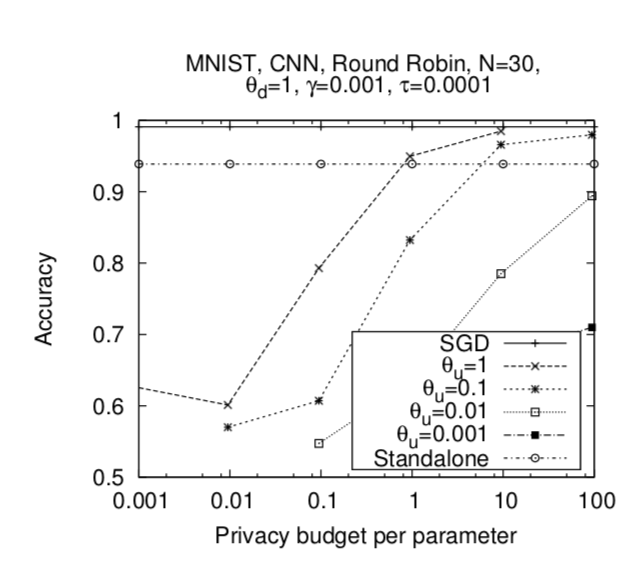
\includegraphics[width = 1.5in]{fig/ccs15_1}}&
\subfloat[参与者为90人]{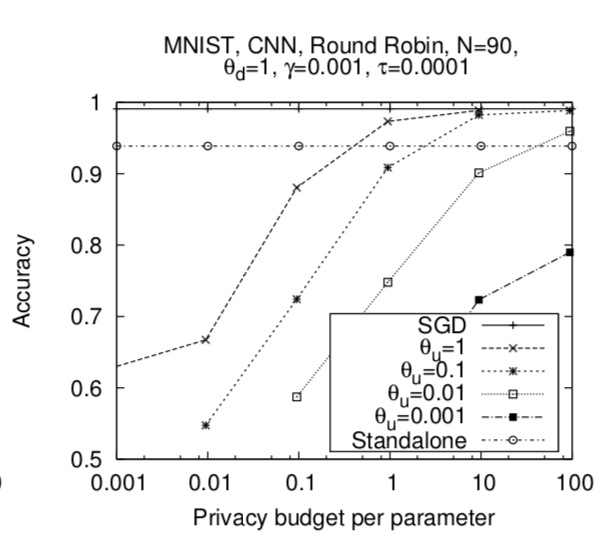
\includegraphics[width = 1.5in]{fig/ccs15_2}}&
\subfloat[参与者为150人]{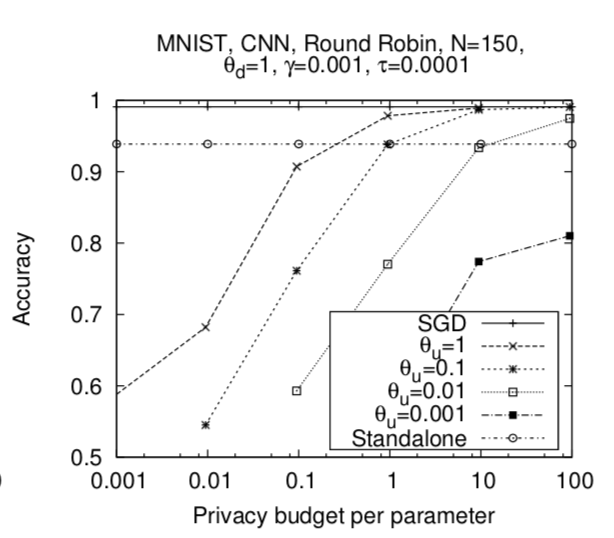
\includegraphics[width = 1.5in]{fig/ccs15_3}}
\end{tabular}
\caption{在MNIST数据集上,对CNN网络的含有差分隐私的协作学习。其中横轴为$\epsilon$,表示差分隐私的强度$\epsilon$越大差分隐私保护添加的噪声越弱。N表示参与者的人数,$\theta_d$表示参数下载的比例,$\theta_u$表示参数上传到比例。从图中可以看出,1:条件相同时参与人数越多准确性越高;2:$\epsilon$越大(噪声越小)准确性越高;3:$\theta_u$越大准确性越高。}
\label{fig:CCS15}
\end{figure}
\end{frame}

\begin{frame}{相关工作}{同态加密}
\begin{enumerate}
\item 2017年,Phong等人在TIFS'17上发表了文章\cite{Phong2017PrivacyPreservingDL}\footfullcite{Phong2017PrivacyPreservingDL},对\cite{shokri2015privacy}提出的协作学习模型的安全及隐私性进行分析,并提出使用同态加密的方法来加密上传给服务器的梯度(gradients)。
\item 为了进一步确保在上传给服务器的同态加密密文的完整性,在于服务器的通讯中采用TLS/SSL安全信道。
\item 一方面,对上传的梯度使用基于LWE或者Paillier的同态加密会增加参与者与服务器之间的通讯开销,但实验表明增加的通讯开销量还是可接受的;
\item 另一方面,相比于\cite{shokri2015privacy}中使用差分隐私减少了一部分准确性来说,计算量的增加带来效率的降低还是可以接受的,因为毕竟在深度学习领域准确性比效率更重要。
\end{enumerate}
\end{frame}

\begin{frame}{相关工作}{同态加密}
\begin{figure}[!ht]
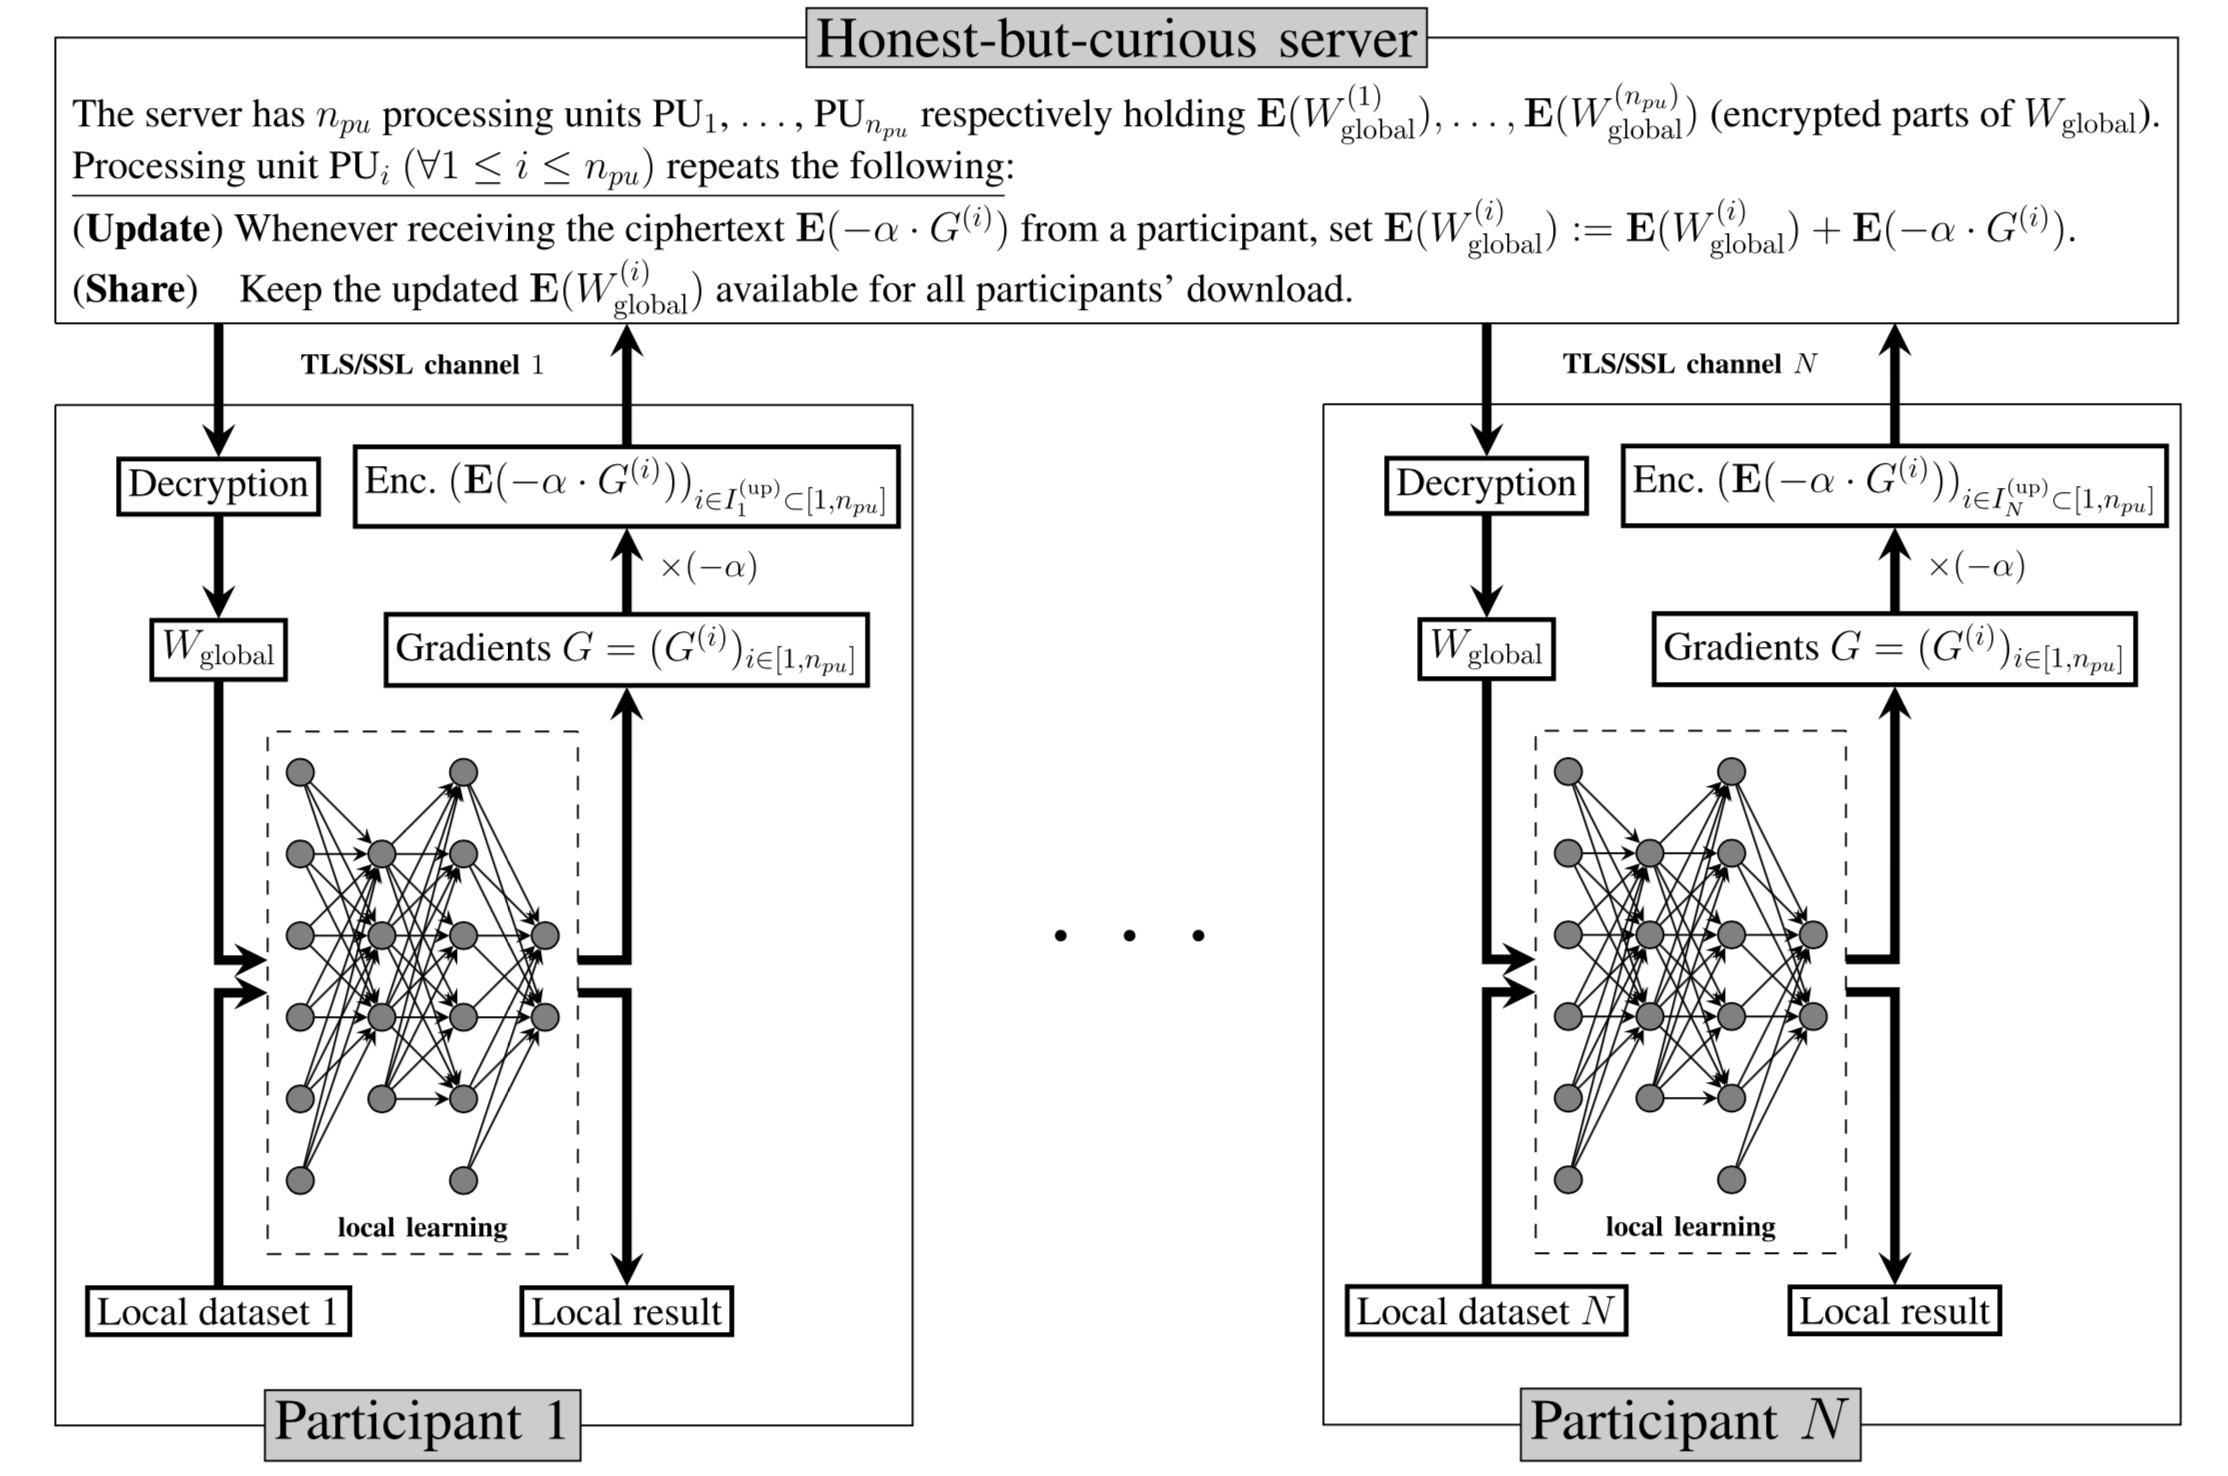
\includegraphics[width = 3in]{fig/TIFS17.png}
\caption{使用同态加密的协作学习模型}
\label{fig:TIFS17}
\end{figure}
\end{frame}

\section{攻击}
\begin{frame}{攻击}{介绍}
\begin{itemize}
\item \cite{Phong2017PrivacyPreservingDL}考虑的是服务器是恶意的,有可能窃取参与者的训练数据。
\item Hitaj等人在CCS'17上发表了一篇关于协作学习中参与者隐私泄露的文章\cite{hitaj2017deep},考虑的是参与者有可能是active的Adversary,从而获取到其他参与者的训练数据。
\item 文章\cite{hitaj2017deep}对\cite{shokri2015privacy}中提出的协作学习进行了攻击,通过使用对抗生成网络(GAN)成功地从其中某个参与者中获得了训练数据\footfullcite{hitaj2017deep}。
\item 进一步地,即使在将参数上传至服务器之前使用差分隐私在参数中加入噪声,只要差分隐私的粒度是record-level的,攻击仍然可以成功。
\end{itemize}
\end{frame}

\begin{frame}{攻击}{介绍}
\begin{itemize}
\item 黑盒攻击:在模型训练完后对模型进行攻击(无需考虑训练过程):
	\begin{enumerate}
 	\item Model extraction attacks
 	\item Model inversion attacks
 	\item Membership inference attacks
 	\end{enumerate}
\item 这是一种白盒攻击:在模型训练阶段攻击,攻击者像其他参与者一样参与到模型的训练中,可以看到并使用模型的参数。
\item 另一方面,攻击者会偷偷地使用其他参与者共享的参数使用GAN网络生成与受害者训练数据类似的数据,每一次迭代攻击者都可以获取到更多受害者的训练数据,最后攻击者可以完整的还原出受害者的训练数据,攻击成功。
\item 在这种情况下,只要参与者的本地模型精确度足够高,攻击者都可以成功获取到受害者的原始训练数据。
\end{itemize}
\end{frame}


\begin{frame}{攻击}{介绍}

值得一提的是,\cite{hitaj2017deep}提出的这种攻击方法对于Google的联合学习模型同样有用。
\begin{itemize}
\item 和\cite{shokri2015privacy}使用差分隐私来保护分享的参数不同,联合学习中采用了一种安全聚集协议(secure aggregation protocol)\cite{bonawitz2017practical}\footfullcite{bonawitz2017practical}。
\item 通过使用安全多方计算(MPC)计算模型参数的平均权重,依据权重每个移动设备的更新(updates)都可以被安全地聚集起来,而且这也使得只有在多个用户的参与下Google才能对模型参数进行解密,这样就可以防止Google窃取用户的模型参数。
\item 由于\cite{bonawitz2017practical}的安全模型中也是只考虑了Google可能是Adversary,并没有考虑参与者的任何一个人都可能成为Adversary,进而去攻击其他参与者以获取其训练数据。因此此攻击对于联合学习仍然有效。
\end{itemize}
\end{frame}

\begin{frame}{攻击}{威胁模型}
\begin{itemize}
\item 设$V$为受害者并且有标签$[a,b]$,$A$为敌手且有标签$[b,c]$。
\item $A$的目标就是尽可能推断出更多关于$a$的信息。$A$会使用GAN生成非常类似$a$的样本,然后把它标记成$c$,并在本地训练,并将其模型参数上传至服务器。
\item 这样,$V$需要去在$a$和$c$中辨别真假,就会暴露更多关于$a$的信息。
\end{itemize}
详细步骤如下:
\end{frame}

\begin{frame}{攻击}{威胁模型}
\begin{enumerate}
\item 假设$A$和$V$双方提前对学习结构和目标达成了一致。
\item $V$有标签$[a,b]$,$A$有标签$[b,c]$。
\item 执行协作深度学习协议若干轮,当且仅当参数服务器上的模型和本地的模型都达到特定的准确度才停止迭代。
\item $V$开始训练:
	\begin{enumerate}
	\item $V$从参数服务器上下载部分参数($\theta_d$),并更新本地模型。
	\item $V$在$[a,b]$上训练本地模型。
	\item $V$上传部分本地模型的参数到服务器上。
	\end{enumerate}
\item $A$开始训练:
	\begin{enumerate}
	\item $A$从参数服务器上下载部分参数($\theta_d$),并更新本地模型。
	\item $A$训练本地的GAN来模仿$V$的$a$。
	\item $A$的GAN生成样本,并把它们标记成$c$。
	\item $A$在$[b,c]$上训练本地模型。
	\item $A$上传部分本地模型的参数到服务器上。
	\end{enumerate}
\item 重复步骤4和5,直到模型收敛。
\end{enumerate}

\end{frame}

\begin{frame}{攻击}{威胁模型}
\begin{figure}[!ht]
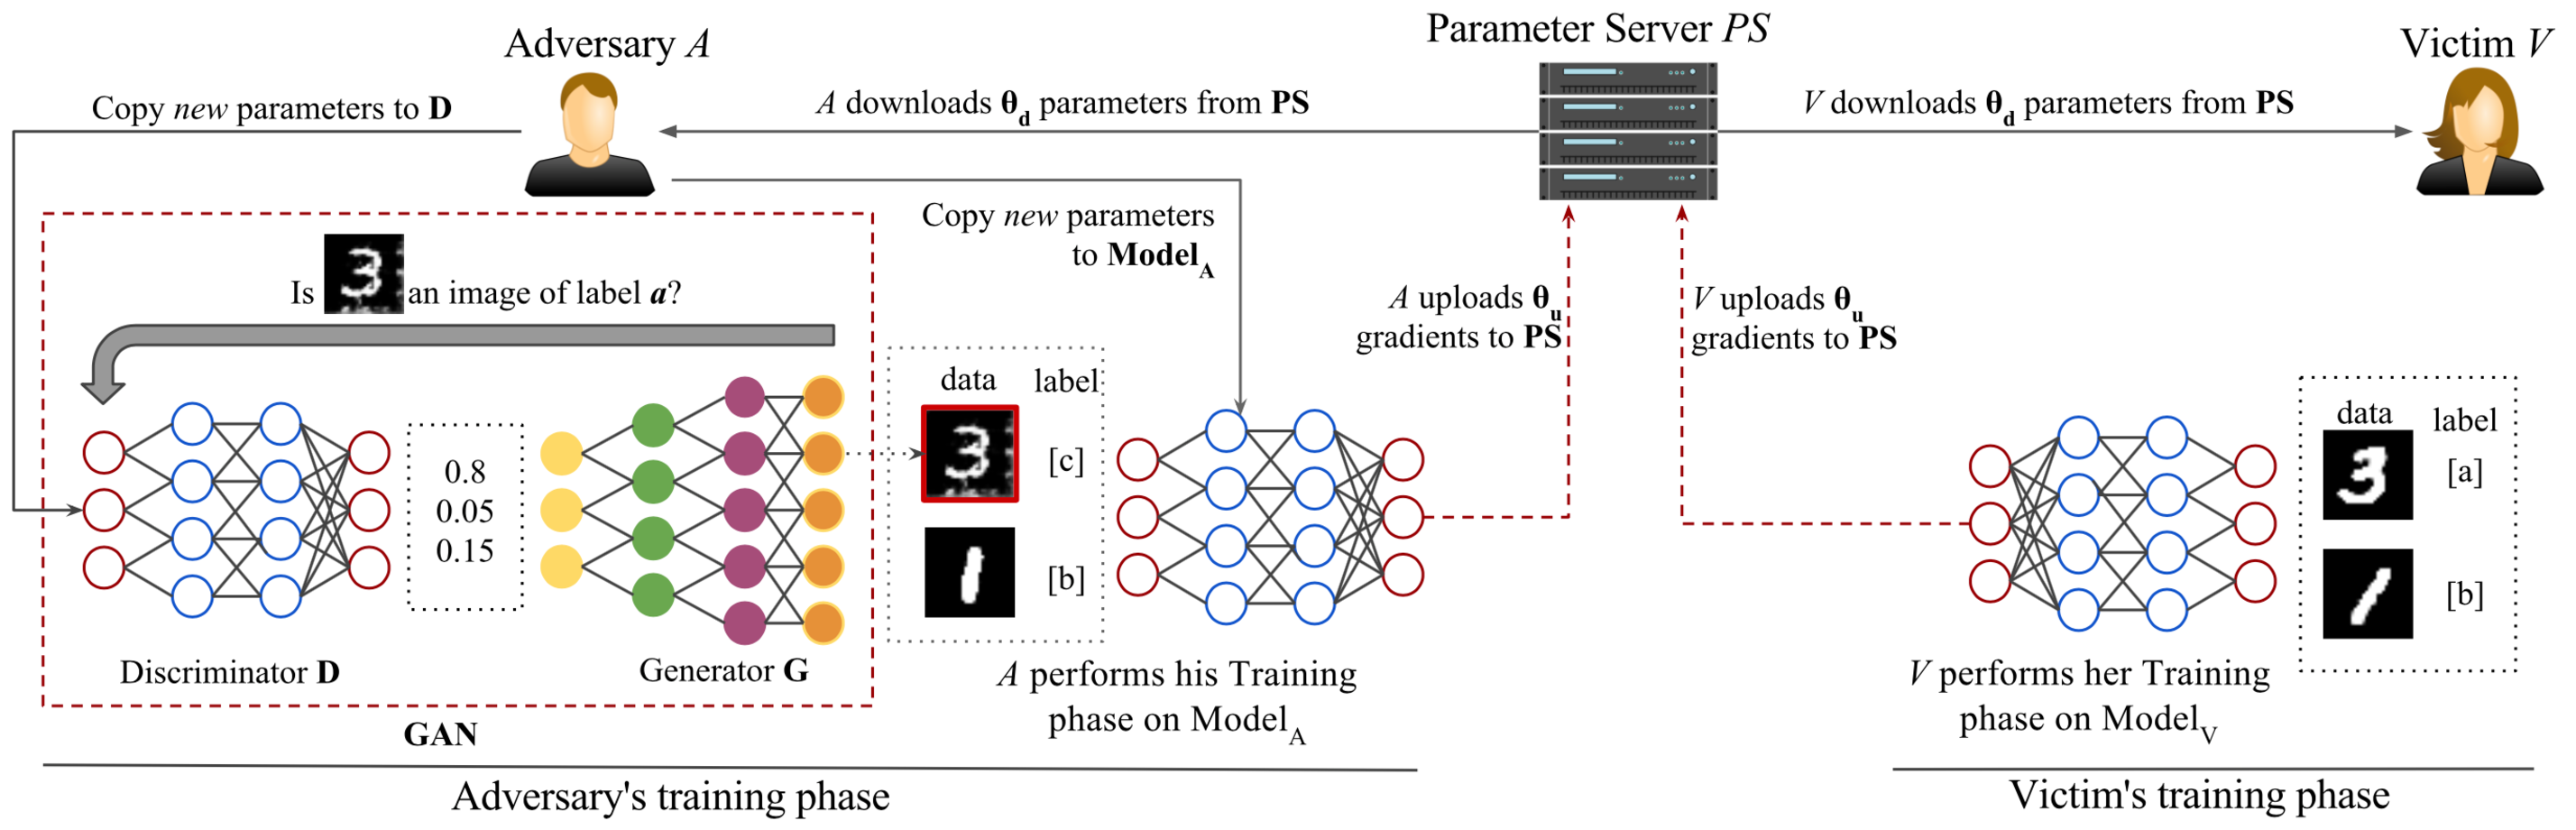
\includegraphics[width = \linewidth]{fig/ganscenario_new.pdf}
\caption{使用GAN攻击正在训练MNIST数据集的协作深度学习模型。}
\label{fig:ganscenario}
\end{figure}
\end{frame}



\begin{frame}{攻击}{实验结果}
\begin{figure}[!ht]
\centering
\setlength{\tabcolsep}{2pt}
\begin{tabular*}{\textwidth}{c c c}
\setlength{\tabcolsep}{1pt}
\subfloat[$\theta_u = 1, \theta_d = 1$]{
\begin{tabular}{lllll}


\includegraphics[width = 0.3in]{fig/original_for_sample_5_400_100.png}  & 
\includegraphics[width = 0.3in]{fig/original_for_sample_5_390_200.png} & 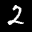
\includegraphics[width = 0.3in]{fig/original_for_sample_5_500_300.png} & 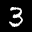
\includegraphics[width = 0.3in]{fig/original_for_sample_5_480_400.png} & 
\includegraphics[width = 0.3in]{fig/original_for_sample_5_400_500.png} \\ 
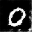
\includegraphics[width = 0.3in]{fig/sample_5_epoch_400_taskid_100.png}  & 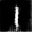
\includegraphics[width = 0.3in]{fig/sample_5_epoch_390_taskid_200.png} & 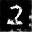
\includegraphics[width = 0.3in]{fig/sample_5_epoch_500_taskid_300.png} & 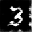
\includegraphics[width = 0.3in]{fig/sample_5_epoch_480_taskid_400.png} & 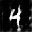
\includegraphics[width = 0.3in]{fig/sample_5_epoch_400_taskid_500.png}  \\
\end{tabular}
}
    &
 \setlength{\tabcolsep}{1pt}
\subfloat[$\theta_u = 0.1, \theta_d = 1$]{
\begin{tabular}{lllll}


\includegraphics[width = 0.3in]{fig/original_for_sample_4_950_0.png}  & 
\includegraphics[width = 0.3in]{fig/original_for_sample_4_960_1.png} & 
\includegraphics[width = 0.3in]{fig/original_for_sample_5_910_3.png} & 
\includegraphics[width = 0.3in]{fig/original_for_sample_5_870_4.png} & 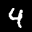
\includegraphics[width = 0.3in]{fig/original_for_sample_5_830_5.png} \\ 
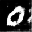
\includegraphics[width = 0.3in]{fig/sample_4_epoch_950_taskid_0.png}  & 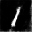
\includegraphics[width = 0.3in]{fig/sample_4_epoch_960_taskid_1.png} & 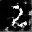
\includegraphics[width = 0.3in]{fig/sample_5_epoch_910_taskid_3.png} & 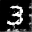
\includegraphics[width = 0.3in]{fig/sample_5_epoch_870_taskid_4.png} & 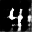
\includegraphics[width = 0.3in]{fig/sample_5_epoch_830_taskid_5.png} \\ 
\end{tabular}
}
    &
 \setlength{\tabcolsep}{1pt}
\subfloat[$\theta_u = 0.1, \theta_d = 0.1$]{
\begin{tabular}{lllll}


\includegraphics[width = 0.3in]{fig/original_for_sample_4_1650_100.png}  & 
\includegraphics[width = 0.3in]{fig/original_for_4_1610_200.png} & 
\includegraphics[width = 0.3in]{fig/original_for_4_1620_300.png} & 
\includegraphics[width = 0.3in]{fig/original_for_sample_4_1620_400.png} & 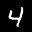
\includegraphics[width = 0.3in]{fig/original_for_sample_5_1950_500.png}\\ 
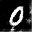
\includegraphics[width = 0.3in]{fig/sample_4_epoch_1650_taskid_100.png}  & 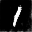
\includegraphics[width = 0.3in]{fig/sample_4_epoch_1610_taskid_200.png} & 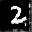
\includegraphics[width = 0.3in]{fig/sample_4_epoch_1620_taskid_300.png} & 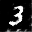
\includegraphics[width = 0.3in]{fig/sample_4_epoch_1620_taskid_400.png} & 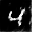
\includegraphics[width = 0.3in]{fig/sample_5_epoch_1950_taskid_500.png} \\ 
\end{tabular}
}
\end{tabular*}
\caption{使用GAN在MNIST数据集上攻击两个参与者场景下的结果。图中下面一行是GAN生成的样本,上面一行是受害者训练集中的数据。其中$(a)$图的参数上传下载比例都是100\%,$(b)$图为10\%,100\%,$(c)$图为10\%,10\%。}
\label{fig:ganresults}
\end{figure}
\end{frame}




\begin{frame}{攻击}{实验结果}
\begin{figure}[!ht]
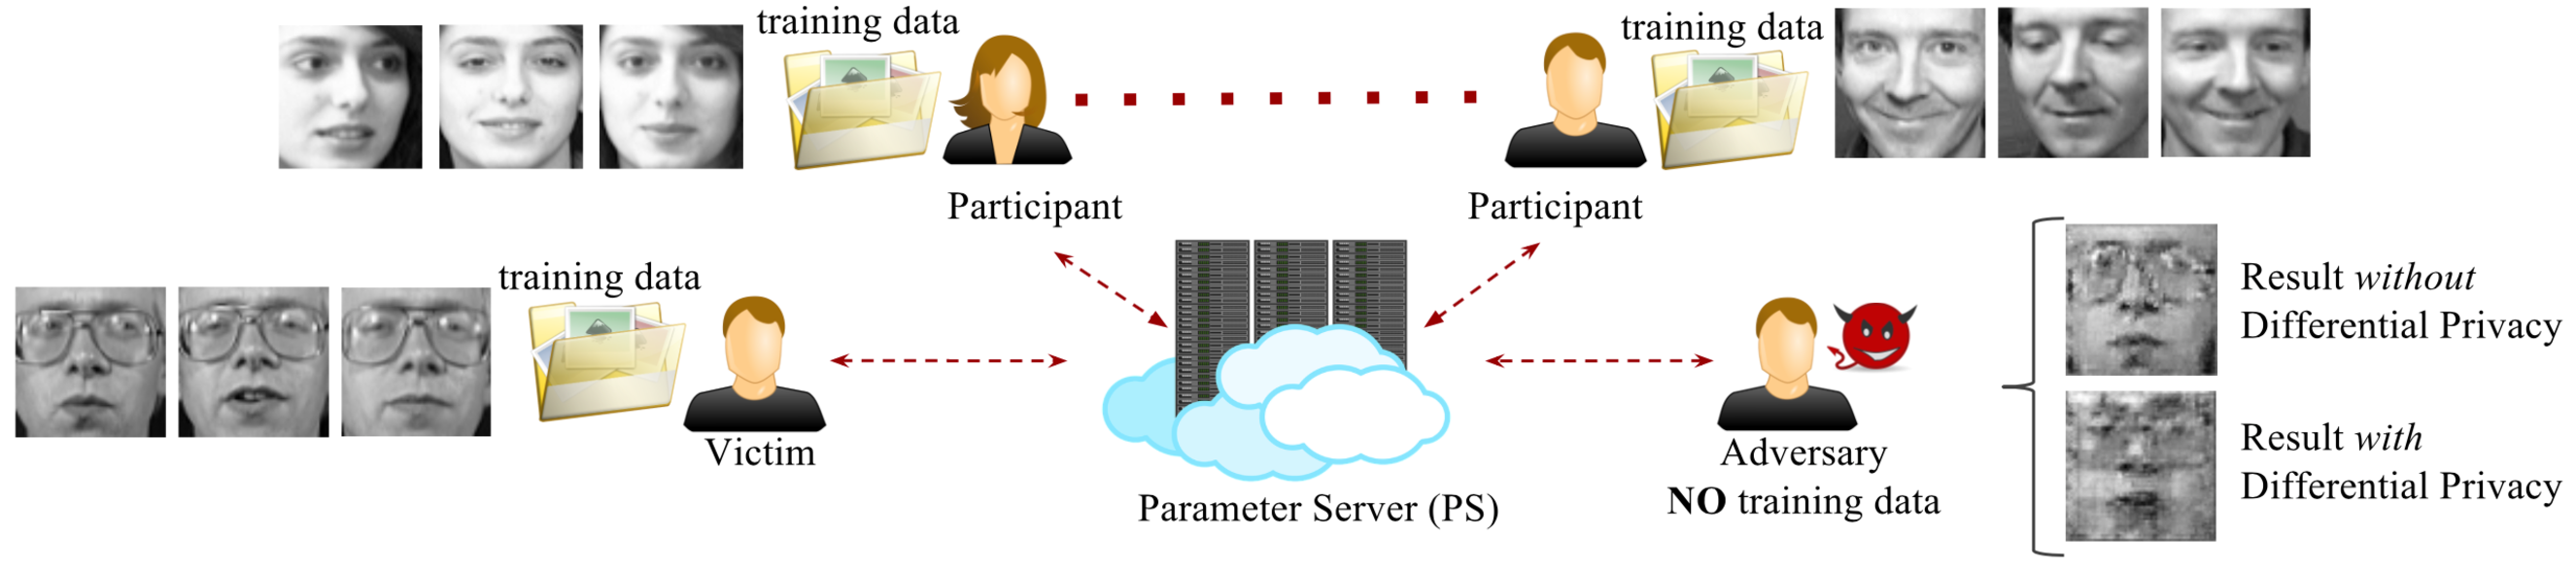
\includegraphics[width = \linewidth]{fig/41_participants.pdf}
\caption{使用GAN在AT\&T的Olivetti人脸数据集上攻击的结果。诚实的参与者们互相独立地训练模型,且敌手$A$并没有本地的训练数据,通过使用GAN攻击,$A$可以重新构建出受害者$V$的训练数据。即使在使用差分隐私的情况下,这种攻击也能成功。}
\label{fig:41_participants}
\end{figure}
\end{frame}

\section{未来工作}
\begin{frame}{未来工作}
因为刚接触深度学习及其隐私问题不久,可能对其了解不够深刻。我想以此工作作为切入点,继续再次详细地看一看本文涉及的paper。一方面持续关注深度学习领域的隐私保护问题,另一方面还要看看目前比较热门的基因技术和机器学习技术的结合点及其隐私保护问题,或者是否可以根据基因数据的特点,将现有的机器学习的隐私保护方案用到基因数据的隐私保护方面。
\end{frame}


\begin{frame}{References}
\printbibliography
\end{frame}
\end{document}














